\documentclass [12pt]{article}
\usepackage{epsfig}
\usepackage{enumitem}
\usepackage{amsmath}
% \usepackage{mathtools}
\usepackage{amssymb}
% \usepackage{amsthm}
% \usepackage{amscd,amsxtra,latexsym}
% \usepackage[color, leftbars]{changebar}
% \usepackage{fontawesome} 
% \usepackage{caption}
% \usepackage{subcaption}

%%%%%%%%%%%%%%%%%%%%%%%%%%%%%%%%%%%%%%%%%%%%%%%%%%%%%%%%%%%%%%%%%%%%%%%%
\usepackage{xcolor}
%% https://tex.stackexchange.com/questions/401750/quick-and-short-command-for-coloring-one-word
\newcommand\shorthandon{\catcode`@=\active \catcode`^=\active \catcode`*=\active }
\newcommand\shorthandoff{\catcode`@=12 \catcode`^=7 \catcode`*=12 }
\shorthandon
\def@#1@{\textcolor{red}{#1}}%
\def^#1^{\textcolor{blue}{#1}}%
\def*#1{\string#1}
\shorthandoff
%% useage: \textcolor{red}{text here}
% \shorthandon
% This is a @test@ of the ^emergency^ bro*@dcast system.
% \shorthandoff
%%%%%%%%%%%%%%%%%%%%%%%%%%%%%%%%%%%%%%%%%%%%%%%%%%%%%%%%%%%%%%%%%%%%%%%%



\setlength{\textwidth}{6.5in}
\setlength{\textheight}{9in}
\setlength{\oddsidemargin}{0in}
\setlength{\evensidemargin}{0in}
\setlength{\topmargin}{-0.5in}

\setlength{\parindent}{0pt}


\newlength{\toppush}
\setlength{\toppush}{2\headheight}
\addtolength{\toppush}{\headsep}

\usepackage{hyperref}
\hypersetup{
    colorlinks=true,
    linkcolor=blue, % was previously black
    filecolor=magenta,
    urlcolor=blue,
    pdftitle={Template}
}
\urlstyle{same}


\def\subjnum{EE 156}
\def\subjname{Adv. Comp. Arch.}

\def\doheading#1#2#3{\vfill\eject\vspace*{-\toppush}%
  \vbox{\hbox to\textwidth{{\bf} \subjnum: \subjname \hfil Amy Bui}%
    \hbox to\textwidth{{\bf} Tufts University, Spring 2023 \hfil#3\strut}%
    \hrule}}

\newcommand{\htitle}[1]{\vspace*{3.25ex plus 1ex minus .2ex}%
\begin{center}
{\large\bf #1}
\end{center}} 

%%%%%%%%%%%%%%%%%%%%%%%%%%%%%%%%%%%%%%%%%%%%%%%%%%%%%%%%%%%%%%%%%%%

\begin{document}
\doheading{2}{title}{Reading Notes}
\htitle{Quantum Computer Systems} 
% \bigskip 
% \bigskip 
%%%%%%%%%% begin text after this line %%%%%%%%%%%%%%
    %%%%%%%%%%%%%%%%%%%%%%%%%%%%%%%%%%%%%%%%%%%%%%%%%%%%%%%%%%%%%%%%%%%%%%%%
    % Table of Contents
    \setcounter{tocdepth}{3}
    \tableofcontents
    % \pagebreak
    %%%%%%%%%%%%%%%%%%%%%%%%%%%%%%%%%%%%%%%%%%%%%%%%%%%%%%%%%%%%%%%%%%%%%%%%

    \begin{thebibliography}{1}
        \bibitem[1]{book}Y. Ding, F. Chong. \href{https://link.springer.com/book/10.1007/978-3-031-01765-0}{Quantum Computer Systems: Research for Noisy Intermediate-Scale Quantum Computers}. Springer Cham. Synthesis Lectures on Computer Architecture. 2020
        \bibitem[2]{vids}\href{https://www.youtube.com/watch?v=7kb1VT0J3DE&ab_channel=CrashCourse}{Crash Course: QM 1/2}, \href{https://www.youtube.com/watch?v=qO_W70VegbQ&ab_channel=CrashCourse}{Crash Course: QM 2/2}, \href{https://www.youtube.com/watch?v=JhHMJCUmq28}{QC Explained}, \href{https://www.youtube.com/watch?v=jHoEjvuPoB8}{QC w/QP}, \href{https://www.youtube.com/watch?v=g_IaVepNDT4&ab_channel=Veritasium}{How QC works (Qubits)}
        \bibitem[3]{wiki}\href{https://en.wikipedia.org/wiki/Quantum_computing}{Wiki: QC}, \href{https://en.wikipedia.org/wiki/Quantum_logic_gate}{Wiki: Quantum Logic Gates}, \href{https://en.wikipedia.org/wiki/Quantum_tunnelling}{Wiki: Quantum Tunneling}, \href{https://en.wikipedia.org/wiki/Quantum_superposition}{Quantum Superposition}
        \bibitem[4]{scqb}Morten Kjaergaard, Mollie E. Schwartz, Jochen Braumüller, Philip Krantz, Joel I.-J. Wang, Simon Gustavsson, William D. Oliver. \href{https://www.annualreviews.org/doi/abs/10.1146/annurev-conmatphys-031119-050605}{Superconducting Qubits: Current State of Play}. Annual Review of Condensed Matter Physics 2020 11:1, 369-395
    \end{thebibliography}

    %%%%%%%%%%%%%%%%%%%%%%%%%%%%%%%%%%%%%%%%%%%%%%%%%%%%%%%%%%%%%%%%%%%%%%%%%
    \section{Intro}
    \label{sec:intro}

    \begin{itemize}
        % \item There was a problem in the study of quantum mechanics, where simulating material and chemical processes was done by predicting behavior of elementart particles, like electrons and nuclei. These simulations are unfeasible on traditional computers, because they could not model the staggering number of all possible arrangements of electrons on a small molecule. 

        \item Simulating models of quantum mechanics (i.e. behaviors of elementary particles) is unfeasible on traditional computers because of the staggering number of all posible arragements of electrons on small molecules. 
        
        \item Advances iin quantum chip manufacturing has given us small- and intermediate-scale quantum computer prototypes. This era where quantum computers are large and reliable enough to perform small computational tasks, i.e. the Noisy Intermediate-Scale Quantum (NISQ, John Preskill).
        
        \item The goal of quantum computers is to run real-world applications that classical computers have a hard time solving efficiently. 
        
        \textcolor{red}{When we are going complexity analysis on a program or algorithm, has it always been in the context of classical computer models? How does complexity analysis change for quantum computing models?}
        
        \item Quantum computing/\textbf{quantum algorithms}: 
            \begin{itemize}
                \item only computing model not bound by Church-Turing thesis on computability, i.e. a function on $\mathbb{N}$ can be computed if and only if it is computable by a Turing machine. All computers can only be probabilistically faster than a Turing machine, but a quantum computer can solve computational tasks more efficiently than what was allowed in classical computation and complexity theory.
                \item Computational problems implemented appropriately on a quantum computer can be solved exponentially faster than classical computers (Fourier sampling, factoring large integers, discrete logarithms, cryptography that relies on prime factorization (Shor's algorithm), unstructured database search).
            \end{itemize}
        
        \item  \textbf{Quantum Computer (QC)}: 
            \begin{itemize}
                \item A QC is a computing device that stores information in quantum bits (\textbf{qubits}), rather than traditional bits.
                \item Qubits are transformed by exploiting properties found in \href{https://www.britannica.com/science/quantum-mechanics-physics}{quantum mechanics}. The behaviors of quantum mechanical systems, where particles are at very small energy and distant scales (i.e. atomic and subatomic), are explained by quantum mechanic theory. 
            \end{itemize}

            \textcolor{red}{I still don't understand how quantum mechanics theory translate into computational behavior in hardware? Is behavior now just based on formulas found in quantum mechanics? Is that not also computationally expensivein hardware and software?}

            \begin{itemize}
                \item Traditional digital computers store information in sequences of 0 and 1 bits, and communication is handled by sending the sequence as electrical signals thorugh integrated circuits. Our computers can handle billions of instructions per second because this process is deterministic and fast. 
            \end{itemize}
        
        \item Models of Quantum Computing (QC)
            \begin{description}
                \item[Analog]: the state of a quantum system evolves gradually/\emph{slowly} using quantum operations that \emph{smoothly} changes the system. Resultant information encoded in the final system corresponds (with high probability) to the desired answer. 
                    \begin{itemize}
                        \item The slow evolution of a quantum system allows it to remain at ground state energy. This approach is called an Adiabatic Quantum Computing. 
                        \item Quantum annealing is when these restrictions are lifted and a quantum system is allowed to interact with the thermal environment. 
                        \item Unclear if quantum annealing devices exist that can achieve universal quantum computation or speedups. 
                    \end{itemize}

                \item[Digital Gate-Based]: information is encoded onto a \emph{discrete} and finite set of \emph{qubits} and quantum operations are broken down into a sequence of a few basic \emph{quantum logic gate}s. The correct answer is given by digital measurement outcoms of the qubits. 
                    \begin{itemize}
                        \item Digital QC is more sensitive to noise than Analog QC; noise is non-negligible, and requires noise mitigating techniques to protect the information from qubit decoherence, imprecise control, and manufacturing defects. 
                        \item Discretization allows for discretization of errors and use of redundancy to encode information.
                        \item NISQ digital quantum computers are QCs that deal with noise in this way.
                    \end{itemize}
                
                 
                \item[Measurement-Based]: a universal quantum computation model. Qubits are initialized in a cluster state, and computation involves measuring the qubits in the cluster state. Some measurements are possibly conditioned on the previous measurment outcomes of qubits. Each measurement accomplishes a quantum gate due to gate teleportation. 
            \end{description}

        \textcolor{red}{So is this just using quantum mechanic models in order to arrive at a solution quickly and with a high probability of being the ``right'' solution?}
        
        \item  \textbf{Quantum Processor Unit (QPU) for Classical Computers}
            \begin{itemize}
                \item QC hardware is referred to as QPU because it is envisioned as a hardware accelerator (or co-processor) for classical computers; similar in purpose to a GPU, a QPU's purpose is to deal with quantum information.
                \item QPU does not fetch data or instructions on its own like a GPU. 
                \item Architecture of Quantum Computer Systems is expected to rely on classical processing and classical control. 
            \end{itemize}

            \begin{figure}
                \centering
                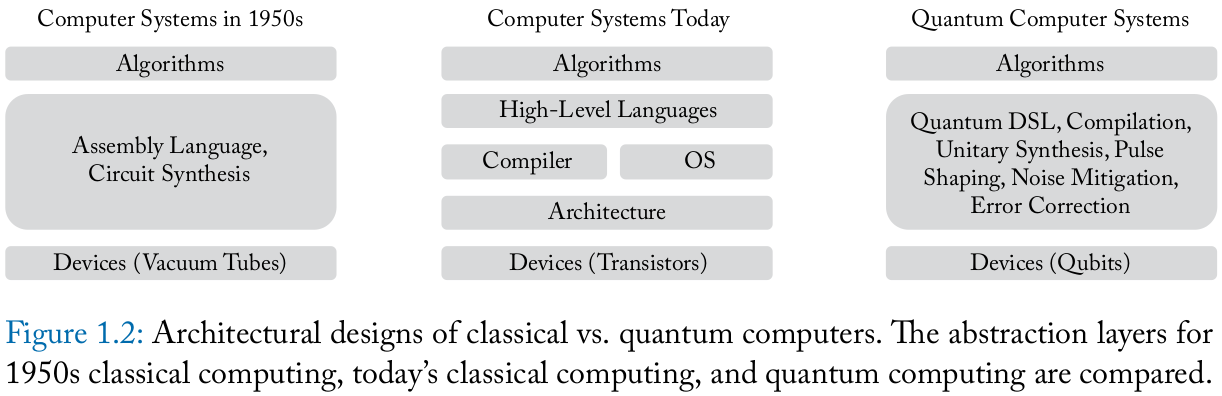
\includegraphics[width=\textwidth]{images/architecturalDesignComparison.png}
            \end{figure}

            \begin{itemize}
                \item In the NISQ era, a QCS cannot copy the layers of abstraction of conventional computer systems (middle); which is why they look like the designs of the 1950s computers, when resources were more strained. Quantum computers are physically large, expensive to make, limited in number of computing units, and demanding on power, just like how early computers were for their time period. NISQ era QCs have 50-1000 qubits, and optimizations are focused on every bit of the limited resources. 
                \item Conventional computers aim to supress the noises caused by quantum mechanics in the transistor components (because they are so small); Quantum computers aim to harness the powers of quantum mechanics. The control apparatuses are fundamentally different between QCS and classical systems. 
                \item Tradeoffs and areas of optimization are reliably addressing and controlling qubits and correcting errors. 
                \item Classical computers are needed to control and assist quantum processors because control complexity becomes overwhelming as the number of qubits scale up; system-level automation can guarantee successful execution of quantum programs. 
            \end{itemize}

            \begin{figure}[htb!]
                \centering
                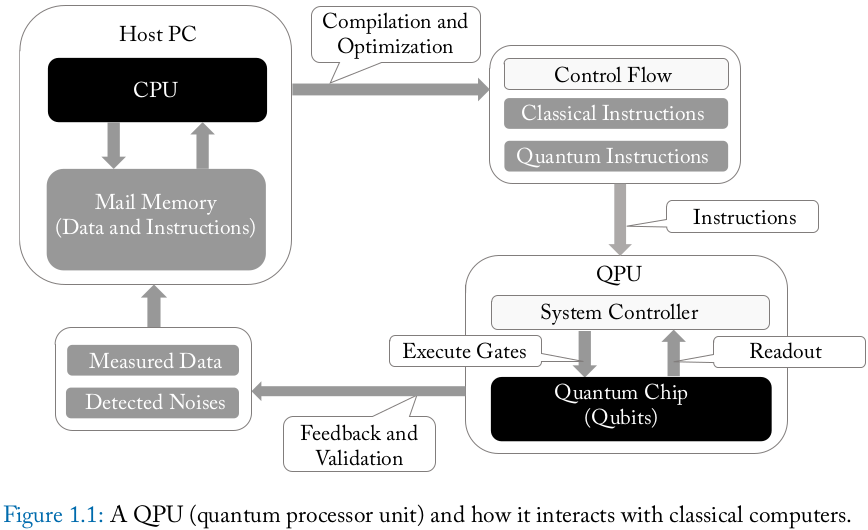
\includegraphics[width=0.7\textwidth]{images/qpuarch.png}
            \end{figure}
        
        \item \textbf{Quantum Technologies} include more than just quantum computation.
            % \begin{itemize}
            %     \item 
            % \end{itemize}
        
        \item It is belived we will see similar scaling in quantum computers as to how 1960s Moore's Law predicted the growth of digital computers. \href{https://en.wikipedia.org/wiki/Robert_J._Schoelkopf}{Schoelkopf's Law} predicts an exponential increase for superconducting qubits based on reported qubit coherence times (lifetimes).
        
        \item \textbf{Qubits}
                \begin{itemize}
                    \item Every qubit doubles the computational space in which quantum machine operates. 
                    \item Qubit resources are limited in today's technology. The quantum machines today have high error rates and will likely for some time until qubit resources catch up. Other areas of study to prepare for such a future include:
                        \begin{itemize}
                            \item The theory of quantum error correction codes will ideally (in the long term) support error-free quantum computations.
                            \item error-tolerant algorithms, correctness of quentum algorithms. 
                            \item lightweight error-mitigating techniques. 
                            \item effects of noise on performance 
                        \end{itemize}
                \end{itemize}
        \begin{figure}[htb!]
            \centering
            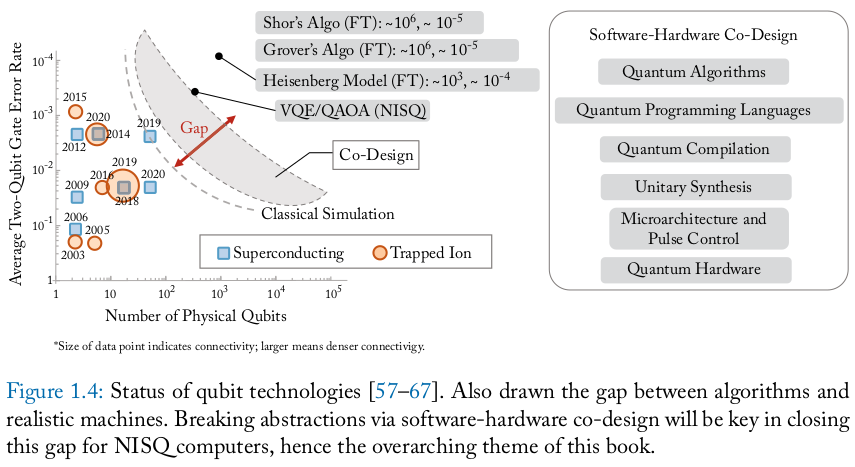
\includegraphics[width=0.7\textwidth]{images/qubittech.png}
        \end{figure}
        
        
        \item Theoretical advances and quantum algorithms are at a point far ahead of where the current technology is. There is a gap between the machines we expect and the algorithms necessary to make full use of their power. Schor's algorithm and Grover's algorithm, for example, require machines much larger than what is currently practical; even smaller-scale quantum algorithms suffer from this gap. 
         
        \item  Software-architecture stack may close the gap with automated optimizations and co-design. The automation will also scale well when quantum programs scale up. 
        
        % \item    
        
        % \item    
        
    \end{itemize}

    %%%%%%%%%%%%%%%%%%%%%%%%%%%%%%%%%%%%%%%%%%%%%%%%%%%%%%%%%%%%%%%%%%%%%%%%%

    %%%%%%%%%%%%%%%%%%%%%%%%%%%%%%%%%%%%%%%%%%%%%%%%%%%%%%%%%%%%%%%%%%%%%%%%%
    \section{Background}
    \label{sec:background}

    \subsection{Bits v. Qubits}
    \subsubsection{Boolean Circuits}
    \begin{itemize}
        \item Boolean circuit Model of Computation: 
            \begin{itemize}
                \item information is stored and manipulated in bits
                \item any computation can be done as a circuit of boolean logic gates. 
                \item 
            \end{itemize}

        \item  von Neumann Architecture
            \begin{itemize}
                \item cpu(alu/CONTROL UNIT), 
                \item ram 
                \item i/o DEVICES 
                \item eXTERNAL STORAGE
                \item Modern CPUs are implmented in electric circuitry printed on integrate circuits, whose building block's are transistors. 
                \item 
            \end{itemize}
        
        \item  Moore's Law: number of transistors per IC grew exponentially every few years since the 60s. But feature size is trending to a stop at a few nanometers (atomic level, where noises from quantum mechanical processes start changing the system). 
        
        \item  Reversible Computation 
            \begin{itemize}
                \item Quantum computers transform quantum bits reversibly
                \item some bit operations are logically reversible, in that the output state uniquely determines what the input state was. ex. NOT gate. Or time-reversible: transformation done by a reversible circuit can be reverted by applying the inverse transformation, which always exists. 
                \item any Boolean circuit can be transformed into a reversible one, and then a quantum one by implementing a quantum Toffoli gate and replacing each bit with a quantum bit.
                \item 
            \end{itemize}
        
        \item  Randomized Computation 
            \begin{itemize}
                \item the physi- cal world contains randomness, as commonly seen in quantum mechanics
                \item randomness may be unnecessary and we can simulate randomized algorithms as efficiently with deterministic ones
                \item $n$-bit probabilistic system (all $p_b$ values must be non-negative and sum to 1): 
                $$ \sum_{b\in \{0,1\}^n} p_b ~|b \rangle $$

                The physical system is in one of these states. Once the random bits in the system are observed, then the state of the system is changed to reflect what was just learnt (laws of conditional probability).
                
            \end{itemize}
    \end{itemize}

    \subsubsection{Qubits and Quantum Circuit Model}
    \begin{itemize}
        \item  Quantum computing described as either randomized computation or reversible computation, each with extra features/conditions. 
        \item Quantum Circuit Model 
            \begin{itemize}
                \item Quantum system $\psi$ is an $n$-qubit system ($\alpha_b$ is amplitude):
                    $$ |\psi\rangle = \sum_{b\in \{0,1\}^n} \alpha_b ~|b\rangle $$

                    $\alpha_b$ can take any complex numbers, and their sum of squared values is 1. i.e. $ \sum_{b\in\{0,1\}^n} |\alpha_b|^2 = 1 $

                \item \emph{Superposition} : probability distribution across bit-strings. Example superposition state: $$ |\psi\rangle =  \frac{1}{\sqrt{2}} |0\rangle + \frac{1}{\sqrt{2}} |1\rangle $$
                \item \emph{Entanglement} of qubits is the correlation between bits
                \item Note that random bits and quantum bits are fundamentally still different objects
                \item \emph{Measure} (observe) the outcome of a qubit, measure all the qubits at the end of a circuit, just like with random bits. Bit-string $|b\rangle$ is observed with probability $|\alpha_b|^2$
                \item upon measurement, the state of the system collapses to the single classical definite value, and can no longer revert back to the superposition it was before. 
                \item \emph{Hadamard Transformation}: a single-qubit quantum gate: 
                multiple results multiple results
                \begin{equation*}
                    H = \begin{cases}
                        |0\rangle \mapsto \frac{1}{\sqrt{2}} |0\rangle + \frac{1}{\sqrt{2}} |1\rangle , \\
                        |1\rangle \mapsto \frac{1}{\sqrt{2}} |0\rangle - \frac{1}{\sqrt{2}} |1\rangle
                    \end{cases}
                \end{equation*}

                Allowing Hadamard gates in a reversible circuit extends the circuit model over any functions allowed to be commputed on qubits 

                \item QM allows for a class of unitary transformations, not just Hadamrd and Toffoli transformations. 
                \item Amplitudes can interfere constructively (accumulate), or interfere destructively (cancel each other out)
                \item quantum circuit looks like reversible circuit, but the qubits are acted on by quantum gates (unitary transformations. )

            \end{itemize}
        
        \item A qubit is a physical object integrated on the quantum chip (i.e. atom, superconducting gadget, etc.). A gate is pulse signals addressed to qubits (laser beam, microwave pulse, etc. )
        \item Classical arch: a gate is an electric circuite component on the CPU. A bit is a voltage signal along wires sent through gates and switches, 
        
    \end{itemize}
        
        
    \subsubsection{QC: Architectural constraints }
            \begin{enumerate}
                \item Info in quantum state extracted through statistics from measurements. Outcomes are probabilistic, so quantum programs must ensure the desired bit-strings are observed with much higher probability compared to undesired ones. 
                \item No-cloning theorem: can't copy qubits; reads are done through measurements that likely alter data, and writes generally require complex state preparattion routines. Can't implement quantum analog of classical memory hierarchy, so current QC arch proposals generall have that transformations are applied directly to quantum memory. 
                \item entanglement / qubit-qubit interactions: incurs communication costs on quantum algorithms on NISQ machines; qubit-qubit interaction overhead is high. 
                \item NISQ machines highly sensitive to environment and control noise, and qubit decoherence (loss of quantum info) happens naturally from spontaneous loss of energe (loss of phase). These errors can accumulate if noot corrected or mitigated.  
            \end{enumerate}
        

    \subsection{Basic Principles of Quantum Computing (Ideal (noise-free) system)}
        % \textbf{}
        \begin{itemize}
            \item Classical computing as operations under laws of boolean algebra. Quantum computation as operations under laws of linear algebra and probabilistic nature of quantum states. 
            
            \item Behaviors of QC manipulated by quantum logic. QC described in in 4 postulates:
        
            \item \textbf{Quantum States postulate}: defines the superposition of each qubit. 
                \begin{itemize}
                    \item A single-qubit quantum state (a superposition state), $|\psi\rangle$: $$ |\psi\rangle = \binom{\alpha}{\beta} $$
                    \item $\alpha, \beta \in \mathbb{C}$, $|\alpha|^2 + |\beta|^2 = 1$
                    \item $\alpha, \beta$ are amplitudes of quantum state.
                    \item superposition state can be rewritten as linear combination using basis states $|0\rangle = \binom{1}{0}$ and $|1\rangle = \binom{0}{1}$: $$ |\psi\rangle = \alpha|0\rangle + \beta|1\rangle = \alpha\binom{1}{0} + \beta\binom{0}{1} = \binom{\alpha}{\beta} $$
                    \item Computational basis states, $|0\rangle$ and $|1\rangle$, are common. Other states
                        \begin{align*}
                            |0\rangle = \binom{1}{0}\hspace{1cm} & |1\rangle = \binom{0}{1} \\
                            |+\rangle = \frac{1}{\sqrt{2}}(|0\rangle + |1\rangle)\hspace{1cm} & |-\rangle = \frac{1}{\sqrt{2}}(|0\rangle - |1\rangle) \\ 
                            |i\rangle = \frac{1}{\sqrt{2}}(|0\rangle + i |1\rangle)\hspace{1cm} & |-i\rangle = \frac{1}{\sqrt{2}}(|0\rangle - i |1\rangle)
                        \end{align*}
                \end{itemize}
            
            \item \textbf{Composition Postulate of Quantum Systems}: generalizes quantum states to represent system of multiple qubits, and defines formally the entanglement property. 
                \begin{itemize}
                    \item In classical computation, an $n$-bit system has $2^n$ possible states. 
                    \item In quantum computing, from superposition principle, the \emph{joint state} of an $n$-qubit system should be a linear combination of $2^n$ possible basis states. Example,  2-qubit system is lienar combination of 4 basis states: $|\psi\rangle = \alpha|00\rangle + \beta|01\rangle + \gamma|10\rangle + \delta|11\rangle$
                    \item Tensor product $\otimes$ of smaller quantum system makes a larger quantum system:  
                        \begin{align*}
                            |\psi_0\rangle = \sum_j \alpha_j ~|a_j\rangle&\hspace{1cm} |\psi_1\rangle = \sum_k \beta_k ~|b_k\rangle\\
                            |\psi\rangle &= |\psi_0\rangle \otimes |\psi_1\rangle\\ 
                            &=\sum_j \sum_k \alpha_j \beta_k ~(|a_j\rangle \otimes |b_k\rangle)
                        \end{align*}
                    (*Can be written as: $|a_j\rangle \otimes |b_k\rangle \sim |a_j b_k\rangle$)
                    \item Separable (product) states are those that can be written as tensor product of two quantum states. 
                    \item Entangled states are a class of multi-qubit states that can't be written as tensor product of two quantum states. Example, Bell state: $$ |\psi\rangle = \frac{1}{\sqrt{2}} (|00\rangle + |11\rangle)$$
                    \item Qubit quantum state visualized in 3D is the Bloch Sphere: 
                        \begin{figure}[htb!]
                            \centering
                            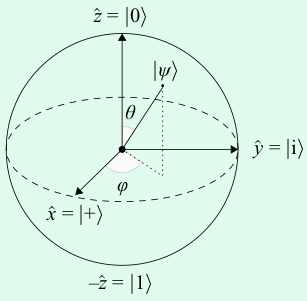
\includegraphics[width=0.3\textwidth]{images/bloch.png}
                        \end{figure}
                        \begin{itemize}
                            \item 1-to-1 mapping from a pure single qubit state $|\psi\rangle$ to a point on surface of Bloch sphere 
                            \item mixed-state is a probability distribution of several pure states, and all mixed states are inside Bloch sphere. 
                            \item No quantum states exist outside the bloch sphere.
                        \end{itemize}


                \end{itemize}
            
            \item \textbf{Measurements postulate}: describes how much info can be read out from a quantum system, and effects of the measurement action to the system
                \begin{itemize}
                    \item The only way to read info out of a quantum system is by interacting with the system via measurement.
                    \item Measurement yields probabilistic outcome. 
                    \item Measuring qubit $|\psi\rangle = \alpha|0\rangle + \beta|1\rangle$, we observe basis state $|0\rangle$ with probability $|\alpha|^2$, and basis state $|1\rangle$ with probability $|\beta|^2$
                    \item Measurement is irreversible and probabilistic. i.e. once measured, $|\psi\rangle$ collapses into one of the two basis states, and the original quantum superposition is not recoverable.
                    \item 
                \end{itemize}
            
            \item \textbf{Quantum Gates postulate}: defines the logical operations that transform a quantum system. 
                \begin{itemize}
                    \item unitary transformation is ``norm-preserving linear transformation''
                    \item to ensure that both $|\psi\rangle, |\phi\rangle$ are valid quantum states, we must have that $|\alpha|^2 + |\beta|^2 = |\alpha'|^2 + |\beta'|^2 = 1$ when transforming $|\psi\rangle = \alpha|0\rangle + \beta|1\rangle$ to $|\phi\rangle = \alpha'|0\rangle + \beta'|1\rangle$
                    \item A valid logical transformation must map one quantum state to another quantum state.
                    \item Logical transformations are deterministic, and they are  reversible, unlike measurement operators. No information is destroyed to leaked to the environment unter unitary transformations.
                    \item Transformation doesn't account for effects of noise. Qubits Decohering to a classical state is incoherent and not reversible. 
                    \item Single-qubit gate is a transformation of one point in bloch sphere to another, by rotating by an arbitrary angle along an axis.
                    \item Multi-qubit gates have an entangling effect. Conditional gate: operation applied to one qubit is dependent on the state of the other qubit.
                    \item 
                \end{itemize}
        \end{itemize}

    \subsection{Noisy Quantum System}
        \begin{itemize}
            \item Quantum systems must involve intentional (e.g. measurements) and unintentional (e.g. random perturbations) incoherence processes. 
            \item probabilistic quantum state applies to niosy quantum system that likely produces a random distribution of quantum states. 
        \end{itemize}

        \subsubsection{Operator Sum Representation (OSR)}
            \begin{itemize}
                \item any physical processes that can happen to a mixed quantum state can be written as a linear map (superoperator): $\rho \mapsto \mathcal{E} (\rho)$
                \item unitary transformation (without interaction with the environment) can be written as an unitary operator: $\mathcal{E} (\rho) = U\rho U^{\dagger}$
                \item $U$ is a unitary transformation.
                \item $U$ acting on both the system and environment (OSR): 
                $$ U(|e\rangle \otimes |\psi \rangle) = \sum_k |e_k\rangle \otimes E_k |\psi\rangle $$
                $$ \mathcal{E} (\rho) = \sum_k E_k \rho E_k^\dagger $$ 
                \item $E_k$ is the Kraus operators
            \end{itemize}

        \subsubsection{Noises}
            \begin{enumerate}
                \item \textbf{Amplitude Damping Noise} $$ \mathcal{E} (\rho) = E_0\rho E_0^\dagger + E_1\rho E_1^\dag  $$
                $$ E_0 = \begin{pmatrix}
                    1 & 0 \\ 
                    0 & \sqrt{1 - \gamma}
                \end{pmatrix} 
                \hspace{1cm}
                E_1 = \begin{pmatrix}
                    0 & \sqrt{\gamma} \\ 
                    0 & 0
                \end{pmatrix}  $$
                    \begin{itemize} 
                        \item quantum system losing energy (spontaneous emission of electrmagnetic radiation for a atom can be modeled as amplitude damping, where $\gamma$ is the probability of emission)
                        \item as time goes by, a quantum state is exponentially more likely to undergo energy loss
                    \end{itemize}

                \item \textbf{Phase Damping Noise} $$ \mathcal{E} (\rho) = E_0\rho E_0^\dagger + E_1\rho E_1^\dag  $$
                $$ E_0 = \begin{pmatrix}
                    1 & 0 \\ 
                    0 & \sqrt{1 - \lambda}
                \end{pmatrix} 
                \hspace{1cm}
                E_1 = \begin{pmatrix}
                    0 & 0 \\ 
                    0 & \sqrt{\lambda}
                \end{pmatrix}  $$
                    \begin{itemize}
                        \item for some $\lambda$ parameter between 0 and 1. 
                        \item Loss of quantum information without loss of energy. 
                        \item process where a qubit undergoes a phase flip (i.e. $Z$ gate) with probability $(1-\sqrt{\lambda})/2$
                    \end{itemize}
                


                \item \textbf{Depolarizing Noise} (stochastic Pauli noise): \textcolor{red}{?}
            \end{enumerate}

    \subsection{Qubit Technologies}
        \begin{itemize}
            \item  Classical equivalent to knowing how qubits work is knowing how transistors work. 
            \item LEaading qubit system technologies today (\textbf{trapped ion qubits, superconducting qubits, semiconductor spin qubits, linear optics, Marjorana qubits, etc.}) have the potential for realizing scalable quantum computing. The book discusses just the first two. 
            \item Qubit design follows Divincenzo Criteria 
                \begin{enumerate}
                    \item scalable system with well organized qubits. 
                    \item ability to initialize qubits  (pprepare in computational basis)
                    \item stability of qubits (long decoherence times)
                    \item support for universal instruction set (single-qubit gates, CNOT, etc) for arbitrary computation 
                    \item ability to measure qubits (readout in computational basis)
                \end{enumerate}
            \item Tradeoffs and difficulty seen in quantum computer designs: initializing, performing gates, and measuring requires interactions between system and environment, but long decoherence times require isolating system from environment. 
            \item Requires a physical system with potential to implement qubitsand that demonstrates scalable architecture. 
        \end{itemize}

        \subsubsection{Architecture: Trapped-Ion Qubits}
            \begin{itemize}
                \item make a qubit with an atomic ion (their internal energy levels exhibit great quantum mechanical properties). Ions are picked because they are charged particles that feel the forces exerted on them by the electromagnetic field. 
                \item Two internal energy levels of an atomic ion (there may be more) represents the quantum states, one for $|0\rangle$ and one for $|1\rangle$
                \item \emph{Optical Qubits}: the two chose energy levels have a separation of $10^{15}$ Hz (in the freq. of visibile light), are from different orbitals (the $s$ and $d$ orbits) of the ion. Common optical qubits include: Ca$^+$ (calcium), Sr$^+$ (strontium), Ba$^+$ (barium), Yb$^+$ (ytterbium) 
                \item \emph{Hyperfine Qubits}: both energy levels are chose from the $s$ orbital of the ion. Energy separation is about  $10^{10}$ Hz (in the microwave spectrum). Common hyperfine qubits are: Ca$^+$ (calcium), Sr$^+$ (strontium), Ba$^+$ (barium), Yb$^+$ (ytterbium), Be$^+$ (beryllium), Mg$^+$ (magnesium), Hg$^+$ (mercury), Cd$^+$ (cadmium), Zn$^+$ (zinc) 
                \item The book references the $^{171}\text{Yb}^+$ (70 protons, 101 neutrons) hyperfine qubit
                \item Measuring trapped-ion hyperfine qubit: state-dependent fluorescence, i.e. excite the qubits in the $|1\rangle$ state $s$ orbit into the $p$ orbit, and measure the transition (decay, which emits photons, which is the fluorescence) back down to the $s$ orbital with the $|0\rangle$ state (lower energy level of the two)
                \item In an QC, a laser beam controls qubits. Lower state electrons are excited to higher states when the laser's frequence matches the separation between the two states (e.g. $10^{10}$ Hz, state transistions controlled by microwave pulses for hyperfine qubits). Pro: low error rates, Con: difficult to focus on individual ions because microwaves are larger wavelengths. Alternatively, state transition via Raman transition, which will excite the electrons to the $p$ orbital/state and decay it back to $s$; con: spontaneous decay can be instantaneous.
                \item 2-qubit gate in a trapped-ion system is is called the XX gate or the Ising gate. Entangling interactions achieved via \href{https://www.chem.purdue.edu/gchelp/liquids/dipdip.html}{dipole-dipole} coupling between two ions.
                \item Ions are trapped in place and prepared to their initial states via \href{https://en.wikipedia.org/wiki/Quadrupole_ion_trap}{RF Paul trap (quadrupole ion trap)} which keeps the ions stationary. 
                \item Trapped-ion QPU, such as the High Optical Access (HOA):
            \end{itemize}

            \begin{figure}[htb!]
                \centering
                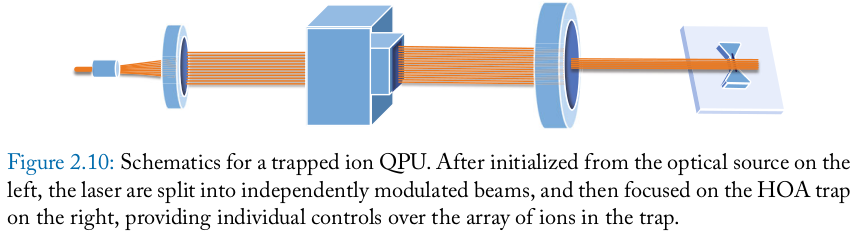
\includegraphics[width=\textwidth]{images/HOA.png}
            \end{figure}

        \subsubsection{Architecture: Superconducting Qubits}
            \begin{itemize}
                \item ``artificial atoms''
                \item implemented with macroscopic, lithographically printed circuit elements, which are parameterized and configured such that they exhibit atom-like energy spectra(``artificial atom'') with desired quantum mechanical properties.
                \item allows convenient design of qubits using existing integrated circuit (IC) technology
                \item \emph{Josephson Junction}: electric circuit element in a superconducting qubit, that is an insulator between two superconductors. It is used to implement an anharmonic oscillator, which has unequal energy spacing. So for computation, we drive transitions between two (lowest) energy levels (represented as qubit states )without exciting other energy levels. Note that the anharmonicity value sets the limit on speed of gate pulses we can apply to a qubit.
                \item pairs of electrons in the superconducting material form bonds, \emph{Cooper pairs}, which have spin of 0 (normal electrons have $\pm \frac{1}{2}$ spin). The cooper pairs can tunnel through the insulator in quantized fashion (one at a time), which gives us the discrete energy levels needed for making a qubit.
                \item \textbf{Superconducting qubit state is related to the number of electrons Cooper pairs tunnelled across the junction.} 
                \item Types of Superconducting Qubits: 
                    \begin{enumerate}
                        \item \textbf{Charge qubit}: computational qubit states defined by the number of Cooper pairs on a superconducting island. Examples: Cooper-pair box qubits, transmon qubits. 
                        \item \textbf{Flux qubit}: superconducting quantum interference device (SQUID) is used instead of a Josephson junction. the energy levels correspond to the integer number of superconducting flux quanta induced in the loop. The book references flux qubits. 
                        \item \textbf{Phase qubit}: computational states are defined using the quantum charge oscillation amplitudes across Josephson junction
                         
                    \end{enumerate}

                    \begin{figure}[htb!]
                        \centering
                        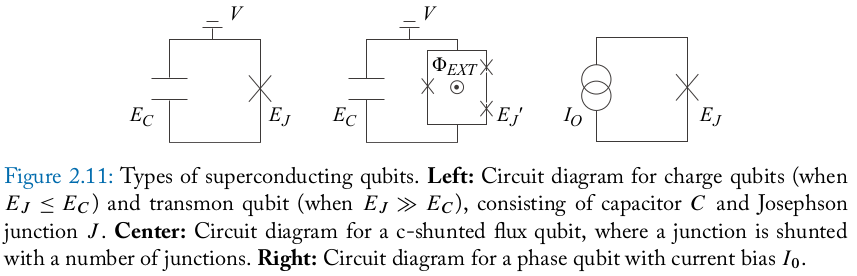
\includegraphics[width=\textwidth]{images/SuperconductingQubits.png}
                    \end{figure}
        
                \item Measurement: Qubit readout done by dispersive readout, which determines qubit state by state-dependent frequency shift of a resonator coupled to each qubit. Changes in the frequency of the resonator can be used to probe qubit state without interacting qith qubit.
                \item Single-Qubit Gates: Two kinds of controls: microwave control (control done by coupling the superconducting qubit to a microwave source (commonly referred to as charge drive or qubit drive) via a capacitor; single-qubti rotation along x and y axis) and flux control (single-qubit rotation along z-axis).
                \item Two-Qubit Gates: interaction between two qubits  is done by tuning the frequencies of the transmons so that the the energy exchange ahppens through capacitive coupling. Ex. resonance.
            \end{itemize}

    \section{Quantum Application Designs: Computational Algorithms QC Can Solve}
        Topics:
        \begin{itemize}
            \item Quantum Information Procesing 
            \item Quantum Parallelism
            \item Quantum Program Cost/Complexity
            \item Algorithms for NISQ
        \end{itemize}

        \subsection{General Features of Quantum Algorithms}
            \begin{itemize}
                \item Quantum computing gives us the ability to encode exponential computational spaceinto just a linear number of computational units, i.e. the state of an $n$-qubit quantum system is represented by $2^n$ complex coefficients. 
                \item Designing quantum algorithms means finding transformations on qubit states that yields a final measuremnt with a high probabilty of the desired outcome. 
                \item Quantum Algorithms generall: 
                    \begin{enumerate}
                        \item efficiently encode info in small number of qubits. 
                        \item cleverly build up entanglement and interference during  the algorithm 
                        \item design a final measurement that yields desired outcome with high probability. 
                    \end{enumerate}
                \begin{figure}[htb!]
                    \centering 
                    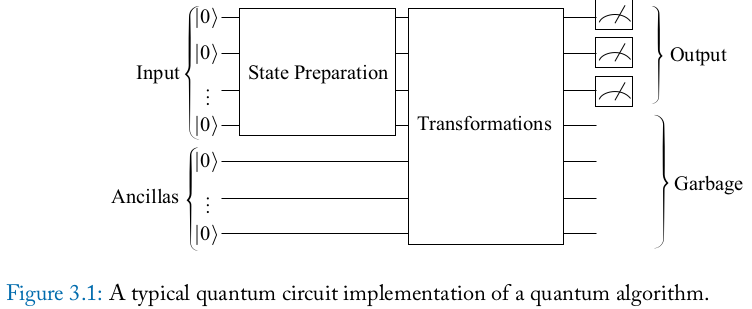
\includegraphics[width=0.7\textwidth]{images/qcircuitqalgo.png}
                \end{figure}
            \end{itemize}
        
        \subsection{Query Model of Computation and Quantum Parallelism}
            \begin{itemize}
                \item Query algorithm is a measuremnt of how to efficiently learn properties of function $f$ (black-box/oracle) of interest. They do so by passing the oracle inputs (query complexity) and analyzing the outputs.
                \item Classical query algorithms only accepts a single input each time. 
                \item Quantum query algorithms can pass several inputs as a superposition quantum state at one time, and then get a new superposition state as output. 
            \end{itemize}
        
        \subsection{Quantum Computational Complexity and Cost}
            \begin{itemize}
                \item Cost is 1) device independent computational complexity, and 2) device-dependent implementation cost. USusally related, i.e. circuit complexity (number of gates) is related to running time (number of steps).
                \item Computational complexity of Quantum Algorithms usually analyzed in time and query complexity 
                    \begin{itemize}
                        \item Time complexity: time complexity of a unitary transformation $U$ is related to the number of gates of the smallest circuit that implements $U$.
                        \item Query complexity: the number of times an algorithm needs to query a given black-box function (often called an oracle) to solve a problem
                    \end{itemize}
                \item The class of BQP (bounded-error quantum polynomial time) decision problems are solvable by polynomia-size uniform quantum circuit family. The relation of BQP to other compuational classes is open problem. 
                \item Implementation Cost: Precision (quantum gates not necessarily accurate due to noise) and resource cost (qubit count, gate count, circuit depth, communication cost, spacetime volume).
                    \begin{enumerate}
                        \item qubit count (circuit width): number of qubit algo needs and the dimensional limits in which the algo can operate. 
                        \item gate count: number of gates an algo needs. Estimate success rate of algorithm, as gate error is dominant noise in NISQ QCs. 
                        \item Circuit depth: number of steps the algo uses, or rather, the deepest path in the circuit from input to output (e.g. ``critical path''). This is related to running time of quantum circuit. Higher circuit depth correlates with lower success rate, because it means more gates (more gate noise), as well as higher likelyhood of qubit decoherence.
                        \item Communication cost: due to physical limits, work must be done to ``communicate'' qubits (closer for interaction/entanglement) to enable actual computation. 
                        \item spacetime volume: ``space $\times$ time'' of algorithm, or rather the quantum volume for a quantum machine is no. qubits $\times$ depth (also error rate and topology). Quantum volume can be used to compare performance to two machines. 
                    \end{enumerate}
            \end{itemize}

            See rest of Ch. 3 for Quantum Algorithms explained in depth. 

    \section{Quantum Systems: Overview}
        \begin{itemize}
            \item  Hybrid approach to quantum-classical co-processing, seen in example theiretical quantum algorithms that still use classical operations with quantum subroutines. 
            \item Quantum Compilers must consider: quantum instruction set, qubit comminucation (fully connected qubit devices are difficult to achieve, and even 2-qubit gates are error-prone), harware noise (memory error from qubit decoherence, gate error from inprecise gate control), and available parallelism.
        \end{itemize}

    \section{Quantum Programming Languages}
        \begin{itemize}
            \item Concepts of data and operations for QC is different than those for classical. 
                \begin{itemize}
                    \item Data (qubit states) is intrinsically probabilistic; Info stored in qubit can only be read out by measurement (irreversible), which yields a probabilistic outcome. 
                    \item Operations on quantum data stored in one part of memory can affect data in another part of memory, due to entanglement. 
                    \item Quantum data cannot be duplicated (no-cloning theorem)
                    \item Quantum states are fragile (sensitive to noise, operational error, and susceptible to decoherence)
                \end{itemize}
            \item Quantum Algorithms typically involve a hybrid of classical and quantum processing
            \item Quantum PL design is approached is to adapt and augment conventional PLs (semantic and typing), to express new properties of quantum programs.
            \item Quantum assembly (QASM) is an early quantum language; it uses a linear sequence of gate instructions to describe programs. (low level, and being sequential makes it difficult to model complex classical control like looping). QASM extensions:
                \begin{itemize}
                    \item Open source: IBM was the first to release a quantum cloud computing, and the QC community has grown substantially 
                    \item OpenQASM is backended by IBM 
                    \item ARTIQ was developed by the trapped ion community
                \end{itemize}
            \item Most (HL) QPL are DSL, which lends itseld well to building off (reusing) existing DSL designs. Its easier, but more general language that adheres closer to quantum information processing theory will help in development of new quantum algorithms. 
            \item Functional QPL:
                \begin{itemize}
                    \item Quipper, Quafl, LIQuI$|\rangle$, Q\#
                \end{itemize}
            \item Imperative QPL:
                \begin{itemize}
                    \item Scaffold (embedded in C/C++)
                    \item ProjectQ 
                    \item Quil (embedded in Python)
                \end{itemize}
            \item Concern in QPL design: lifetime and scaling, because the NISQ systems are rapidly evolving and tools like PL need to keep up, because language, optimizations, compilation, and system design are intertwined. For the most part, quantum algorithms are verified wth mathematical techniques because they are theoretical, so PL is more important for practical, efficient, and correct implementation, rather than new algorithm development. 
            \item QPL design (and the supporting software toolchain) is still new, compared to hardware development and theoretical algorithm understanding. 
        \end{itemize}
        
    \section{Circuit Synthesis and Compilation}
        \begin{itemize}
            \item Quantum Circuit Synthesis Techniques: 
                \begin{itemize}
                    \item choice of universal ISA 
                    \item single-, multi-quibit, qudit synthesis 
                    \item exact and approximate syntesis
                \end{itemize}
            % \item 
        \end{itemize}
        
    % \section{Microarchitecture and Pulse Compilation}
    %     \begin{itemize}
    %         \item 
    %     \end{itemize}

    \section{Noise Mitigation and Error Correction}
        \begin{itemize}
            \item Noise Source Characterization
                \begin{itemize}
                    \item state and process tomography: reconstruct an unknown quantum state from the outcomes of a series of measurements. It is limited in noise estimating of a process dues to SPAM (state preparation and measurement) error. 
                    \item random benchmarking: applying long sequences of gates and postponing measurement to the end in order to address gate error. 
                \end{itemize}
            \item Noise Mitigation can be done with qubit designs that prolong coherence/lifetime, more accurate gate ops, etc.:
                \begin{itemize}
                    \item Randomized compiling: inserting random gates in quantum circuit, converting coherent errors and non-markovian noise into stochastic Pauli errors, which are easier to correct for while preserving the logical operations of the quantum circuit.
                    \item Noise aware mapping: noise in qubits and in gates can vary by the hour. Compilers can take the daily variations into account and optimize using available data on this to increase probabilty of correct outcome. 
                    \item cross talk aware scheduling through: connectivity reduction, qubit frequency tuning, coupler tuning. 
                \end{itemize}
            \item Error Correction (QEC): the goal is to achieve fault-tolerance through redudancy in qubits and turning quantum errors to classical errors. 
            \item 
        \end{itemize}

    % \section{Classical Simulation of QCs}
    %     \begin{itemize}
    %         \item 
    %     \end{itemize}
        
        
    %%%%%%%%%%%%%%%%%%%%%%%%%%%%%%%%%%%%%%%%%%%%%%%%%%%%%%%%%%%%%%%%%%%%%%%%%



%%%%%%%%%%%%%%%%%%%%%%%%%%%%%%%%%%%%%%%%%%%%%%%%%%%%%%%%%%%%%%%%%%%%%%
\end{document}
%%%%%%%%%%%%%%%%%%%%%%%%%%%%%%%%%%%%%%%%%%%%%%%%%%%%%%%%%%%%%%%%%%%%%%

